%-------------------------------------------------------------------------------
\subsection{Validation Phase}
%-------------------------------------------------------------------------------

In order to facilitate atomic committment across all shards involved in a transaction \sys clients invoke a Prepare request, inquiring each shard to validate the transaction for conflicts and cast a 2PC vote. Shards in \sys are replicated for fault tolerance.

\fs{idk where to put this and whether to mention at all - but we do want to state that there exists a version with 3f+1 (minimal replication degree) that implements the same ethos }
\sys comes in two different flavors, \sys{}3 and \sys{}5 respectively, that rely on varying replication degrees, but implement the same design. \sys{}3 requires $n=3f+1$ replicas \fs{, the minimum bound necessary for BFT SMR?,} per shard to guarantee consistency in the presence of $\leq f$ byzantine replicas. \sys{}5 reduces both latencies during failure free execution and complexity during recovery. \footnote{We believe that consortiums with high performance requirements or high replication degrees are respectively comfortable with paying for additional replicas or tolerating a lower fraction (1/3 vs 1/5) of failures}
For the simplicity of exposition we discuss \sys{}5 for the remainder of the paper, and defer to section X \fs{and/or TR} to describe differences in \sys{}3. In the following, we outline \sys 's execution (unaffected by replication degree), validation and writeback protocols.

The goals of the Validation phase are threefold: \one It must decide on a single, durable vote per-shard that maintains Byzantine Serializability (henceforth we refer to this as a \textit{shard-decision}), \two It should be leaderless, and not enforce unecessary ordering for commutative, non-conflicting transactions, and \three It must preserve independent operability. \fs{needs to refer to the fallback}

Satisfying these goals requires ovecoming several challenges. In order to maximize parallelism and embrace partial ordering, \sys allows replicas to process requests out of order. Consequently, replicas may temporarily diverge, and hence return different validation results. Such divergence must be reconciled in a way that maintains Isolation, but not overly conservatively in order to bound the impact of byzantine participants and maximize likehlihood to commit. \sys designates clients as validation coordinator for its own transactions, thus omitting a dedicated replica leader. The respective protocol must tolerate client failures such as crashes, omission/stalling, equivocation, or replays and allow for consistent recovery. 

The Validation protocol can be broken down into two functionalities: Voting and Logging.
Since \sys replicas may process requests in different order, they must reach consensus on a joint  decision. To do so, they cast a vote for their local validation result, which are subsequently democratically aggregated into a decision. In the case of Indicus, the client acts as the transaction coordinator who aggregates and relays results (along with necessary evidence).
In order to maintain consistency in the presence of failures (no two correct replicas finalize different Commit/Abort decisions), this decision must be durable and unique, guaranteeing that a replay of any Writeback is idempotent. However, since a byzantine coordinator cannot be trusted to durably store a decision, nor could we retain liveness during a crash or partition, \sys demands clients to \textit{log} the decision at replicas before returning.
 

The voting step requires a single round-trip to all replicas, whereas the logging phase requires at most one round-trip \fs{in Indicus5 and at most two round-trips in Indicus3.}. When execution is fault- and contention free transactions can be committed on the \textit{Fast-Path} in a single-round trip as an explicit logging round is not necessary.


%%%%%%%%%% protocol
To describe how the protocol operates in detail we follow a single-shard transaction through the system:

\fbox{\begin{minipage}{23em}
\textbf{(1: C $\rightarrow$ R)}: Client sends Prepare request to all Replicas within the Shard.
\end{minipage}}\\
Upon deciding to Commit in the Execution phase, a Client initiates Validation by sending a message $Phase1 \coloneqq \langle Prepare, TxID, TX \rangle_{\sigma_c}$ to all Replicas.

\fbox{\begin{minipage}{23em}
\textbf{(2: R $\rightarrow$ C)}: Replica receives validation request, processes it and returns vote to Client.
\end{minipage}}\\
A replica validates Timestamp and Dependency integrity of the request. It then evaluates Read and Write Sets for Isolation conflicts against its local state using the MVTSO Concurrency Control Check (CCC), as shown in algorithm 1. It returns a message $Phase1R \coloneqq \langle TxID, vote \rangle_r$, and optionally evidence in case it voted to Abort.

\underline{Additional subtlelties}: 
A replica never changes its Voting decision, because re-execution could leave to different results. Once the MVTSO-Ceck completes (i.e. there are no blocking dependencies), a replica starts a timer to monitor the clients progress.

\fbox{\begin{minipage}{23em}
\textbf{(3: C)}: Client waits for vote replies.
\end{minipage}}\\
\fs{re-phrase this: A client does not have to wait for 4f+1, he can return as soon as he sees 3f+1 commits if he wants, or even f+1 aborts if he is impatient.}
A client waits for at least $n-f$ ($4f+1$ in Indicus5) distinct replica votes, or more, up to a system specified timeout. 

\fbox{\begin{minipage}{23em}
\textbf{(3a: C)}: Client receives Threshold of matching votes and returns to application. Proceeds to Writeback
\end{minipage}}\\
In any of the following 3 cases, a client may short-circuit waiting for additional votes and omit a dedicated Logging round:
\begin{enumerate}
\item \textbf{$1$ Abort vote w/ Conflicting TX \& CommitCertificate}: A conflict with a commited transaction. The client validates the integrity of the CommitCertificate and returns the shard decision $(TxID, Abort, \langle ConflTX \rangle_{CC})$. 
\item \textbf{$3f+1$ Abort votes w/ Conflicting TX}: A conflict with a prepared, but not yet committed transaction. The client returns the shard decision $(TxID, Abort, \{\langle AbstainVote\rangle_r\})$. 
\item \textbf{$5f+1$ Commit votes}: No conflicts. The client returns the shard decision $(TxID, Commit, \{\langle CommitVote \rangle_r\}$
\end{enumerate}
Any of such Quorums forms a \textit{Shard-Certificate} and proves the decision. A client uses this Certificate to return to its application and issue the Writeback.

\fbox{\begin{minipage}{23em}
\textbf{(3b: C $\rightarrow$ R)}: Client receives divergent results and suggests a consistent decision to Replicas for Logging
\end{minipage}}\\
If a client does not receive the necessary thresholds of votes to return, it must continue on the \textit{Slow-Path}. To do so, it aggregates the votes according to following decison rule:
If there exists a $CommitQuorum \coloneqq \frac{n+f+1}{2}$ of Commit Votes, the Slow-Path decision is Commit, otherwise it is Abort.
A client broadcasts a message $Phase2 \coloneqq (TxID, decision)_c, \{\langle votes \rangle_r\}$.

\underline{Additional subtlelties}: A client forwards a Quorum of $\geq n-f$ votes to the replicas in order to prove the Slow-Path decision is consistent with Isolation guarantees. Note, that a byzantine client may equivocate the decision by relaying different Quorums.

\fbox{\begin{minipage}{23em}
\textbf{(4: R $\rightarrow$ C)}: Replicas receive, validate and echo decision
\end{minipage}}\\
A replica confirms that the Decision matches the Quorum by evaluating the decision rule itself and adopting the decision. It then returns the decision to the client by sending $Phase2R \coloneqq \langle TxID, decision \rangle_r$. Importantly, a replica never changes its decision.

\fbox{\begin{minipage}{23em}
\textbf{(5: C)}: Client returns shard-decision to application and proceeds to Writeback
\end{minipage}}\\
A client waits for a Quorum of $n-f$ matching $Phase2R$ messages. Such a Quorum forms a \textit{Shard-Certificate} and proves the decision. A client uses this Certificate to return to its application and issue the Writeback.

\underline{Additional subtlelties}: If a client equivocated, it will never receive a Shard-Certificate. A correct client however, is guaranteed to receive matching Phase2 replies. 

We consider a decision (Commit, Abort) to be \textit{logged} when it is possible for some Shard-Certificate to exist, i.e. as soon as the necessary certificate Quorums exists at some Replicas.
Figure \ref{fig:FigureSP} summarizes the relevant nomenclature.

\begin{figure}
\begin{center}
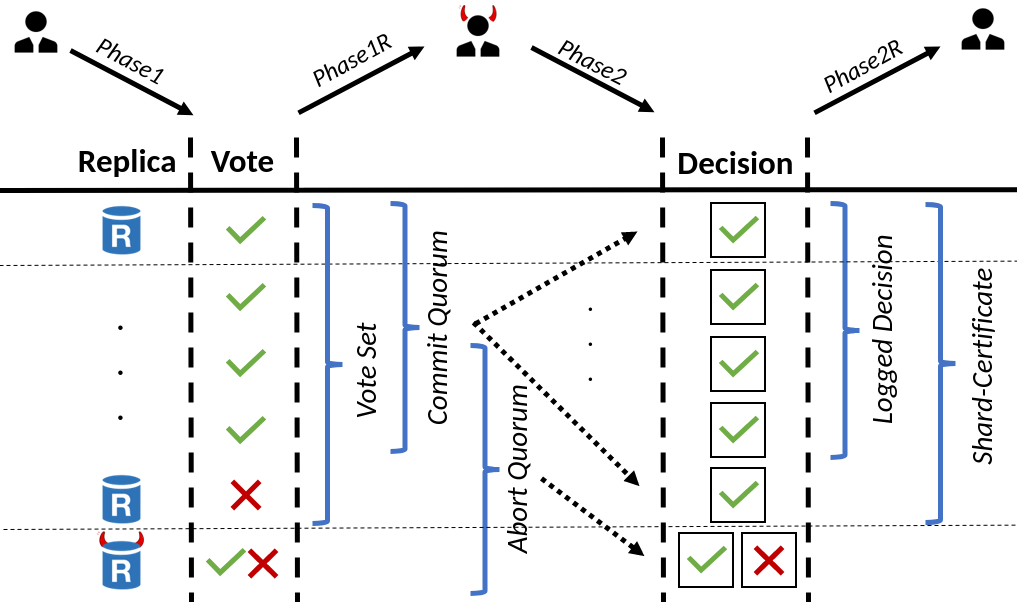
\includegraphics[width= 0.5\textwidth]{./figures/Nom2.png}
\end{center}
\caption{Validation Nomenclature, Slow-Path. Note, that a byzantine client may equivocate Phase2 decisions by including Commit and Abort Quorums respectively. Byantine replicas may store multiple votes and decisions.}
\label{fig:FigureSP}
\end{figure}

\subsubsection{Correctness}
We show, that a \textit{logged} decision is final:
\begin{theorem}[Saf]
A logged decision is durable, and there can ever exist \textbf{at most one} logged decision.
\fs{Clarify the point of this: We preserve consistency of writeback commit/abort. That in turn follows from the logged decision durability.}
\end{theorem}
\begin{proof}
\tr{Proof in Appendix~\ref{}}{Proof in TR~\ref{}}
\iffalse
We show this by case distinction over Slow- and Fast-Path execution. \textbf{Slow-Path}: A Slow-Path decision is \textit{logged} if $\frac{n+f+1}{2} = 3f+1$ ($LoggedQuorum$) correct replicas have adopted the decision, since $n-f = 4f+1$ votes suffice to form a Shard-Certificate and $f$ byzantine participants may decide arbitrarily. Thus it is impossible for two Slow-Path logged decisions to co-exist, as any two $LoggedQuorums$ must intersect in $f+1$ correct replicas that will only ever accept one decision - a contradiction. Furthermore, correct replicas do not change their decision, and hence a slow-path logged decision is durable. \textbf{Fast-Path}: We distinguish three sub-cases. \one A Fast-Path commit shard-certificate requires the existance of $4f+1$ Phase1 correct commit votes. This implies that any Slow-Path execution must result in a commit decision, since there cannot exist $f+1$ Abort votes and client waiting for up to a Vote Set Quorum ($n-f = 4f+1$) is bound to receive $3f+1$ commit votes. \two Vice versa, by Quorum intersection, the existance of $3f+1$ Phase1 abort votes implies the impossibility of any Slow-Path commit decision. 
Trivially, cases \one and \two  mutually exclude each other. 
\three Lastly, 1 Abort vote with valid proof of conflict against a committed transaction implies the existance of a logged commit decision for the conflicting transaction. \fs{Defer this proof to the next theorem... redundant}
By Induction, the conflicting transaction has stored a commit vote or decision at $\geq 3f+1$ correct replicas. Thus, $\geq 3f+1$ correct replicas will vote to Abort the ongoing transaction, hence precluding the existance of $\geq 3f+1$ commit votes and the possibility to ever log a commit decision for the ongoing Transaction.

\fi
\end{proof} 

Note, that since replicas never change their decision, it is possible for there to never be any logged decision if a byzantine client equivocated its Slow-Path Quorums. In order to reconcile this, we design and discuss a recovery mechanism in section X which relaxes the requirement for durability of decisions.  


\begin{theorem} 
Indicus maintains \textit{Byzantine-Serializability}.
\end{theorem}
To prove that this is the case, we show that for any two conflicting transactions, at most one can be committed.
\begin{proof}
\tr{Proof in Appendix~\ref{}}{Proof in TR~\ref{}}
\iffalse
Let $TX_1$ be a transaction with logged decision \textit{Commit}, i.e. $TX_1$ has either already committed at or is bound to commit at all correct replicas. Let $TX_2$ be a conflicting transaction, that if committed would violate Byzantine-Serializability. Assume $TX_2$ too, managed to log a commit decision. By the protocol, at least  $\frac{n+f+1}{2} = 3f+1$ commit votes are required to log a commit decision, and no correct replica changes its vote. By Quorum intersection, at least one correct replica must have voted commit for both $TX_1$ and $TX_2$. WLOG, this replica received $TX_1$ before $TX_2$. By the correctness of the MVTSO-check (\ref{Theorem1}, must have voted Abort for TX2. A contradiction.

\fi
\end{proof}

\begin{theorem} 
Indicus maintains Byzantine Independence in the absence of network adversary.
\end{theorem}

We show, that once a Client submits a transaction for validation, the result cannot be unilaterally decided by any group of (colluding) byzantine participant, be it client or replica.
\begin{proof}
\tr{Proof in Appendix~\ref{}}{Proof in TR~\ref{}}

\iffalse
First, we observe that a client may never autonomously determine a result itself, and may only influence the decision value by choice of Fast- or Slow-Path Quorum. Specifically, a byzantine client cannot single-handedly decide to abort its own transaction once submitted for validation, and consequently, cannot single-handedly force potentially dependent transactions to abort as well. 
Second, any Quorum decision requires at least one correct replicas vote. In particular, $f$ byzantine replicas may arbitrarily vote to abort (e.g. by reactively generating and injecting a ficticious, conflciting transaction), but at least one additional correct replicas' abort vote is necessary to result in an abort decision. 
Thus, in order to artificially cause transactions to abort, a conflicting transaction must be generated (artificial congestion). However, to do so strategically and reliably \fs{deterministically}, the adversary must control the network in order to guarantee the artifical transactions arrival at correct replicas \textit{before} the original transaction. 

Likewise, colluding clients may attempt to abort each other in order to cause a correct clients' dependency to abort. For example, they may attempt to schedule the arrival of two conflicting transactions out of order across replicas. To preemptively setup such a targeted trap however, colluding clients must a) know the to-be-victim transactions read keys, and b) race the respective transaction for arrival order. Doing so deterministically requires control of the network.

Thus, when the network is not adversarial, validation decisions are \textit{Byzantine Independent}.

\fs{need to add the case of dependency trying to get aborted by its own dependent. this too is up to the network: A byz replica does not know that there is a dependent until the exceptions or prepares are being issued. needs to have network control in order to still abort. if there are multiple levels then the colluders could already pre-abort each other: example: out of order at 3 replicas each. any TX coming after that claims a dep is doomed. But this is not deterministic: it requires preemtive setup, but keys are not known}

\fi
\end{proof}









